\section{Roboterarchitektur und Systemkomponenten}

\subsection{Interner Aufbau}
Im Folgenden soll die interne Architektur des \gls{go1} im Detail dargestellt werden.
Hierfür werden einige Perspektiven des Roboters gezeigt, um die nach Einsatzzweck klassifizierten Bauteilgruppen zu erläutern und darzustellen.

\subsubsection{Überblick}

\begin{figure}[h]
    \frame{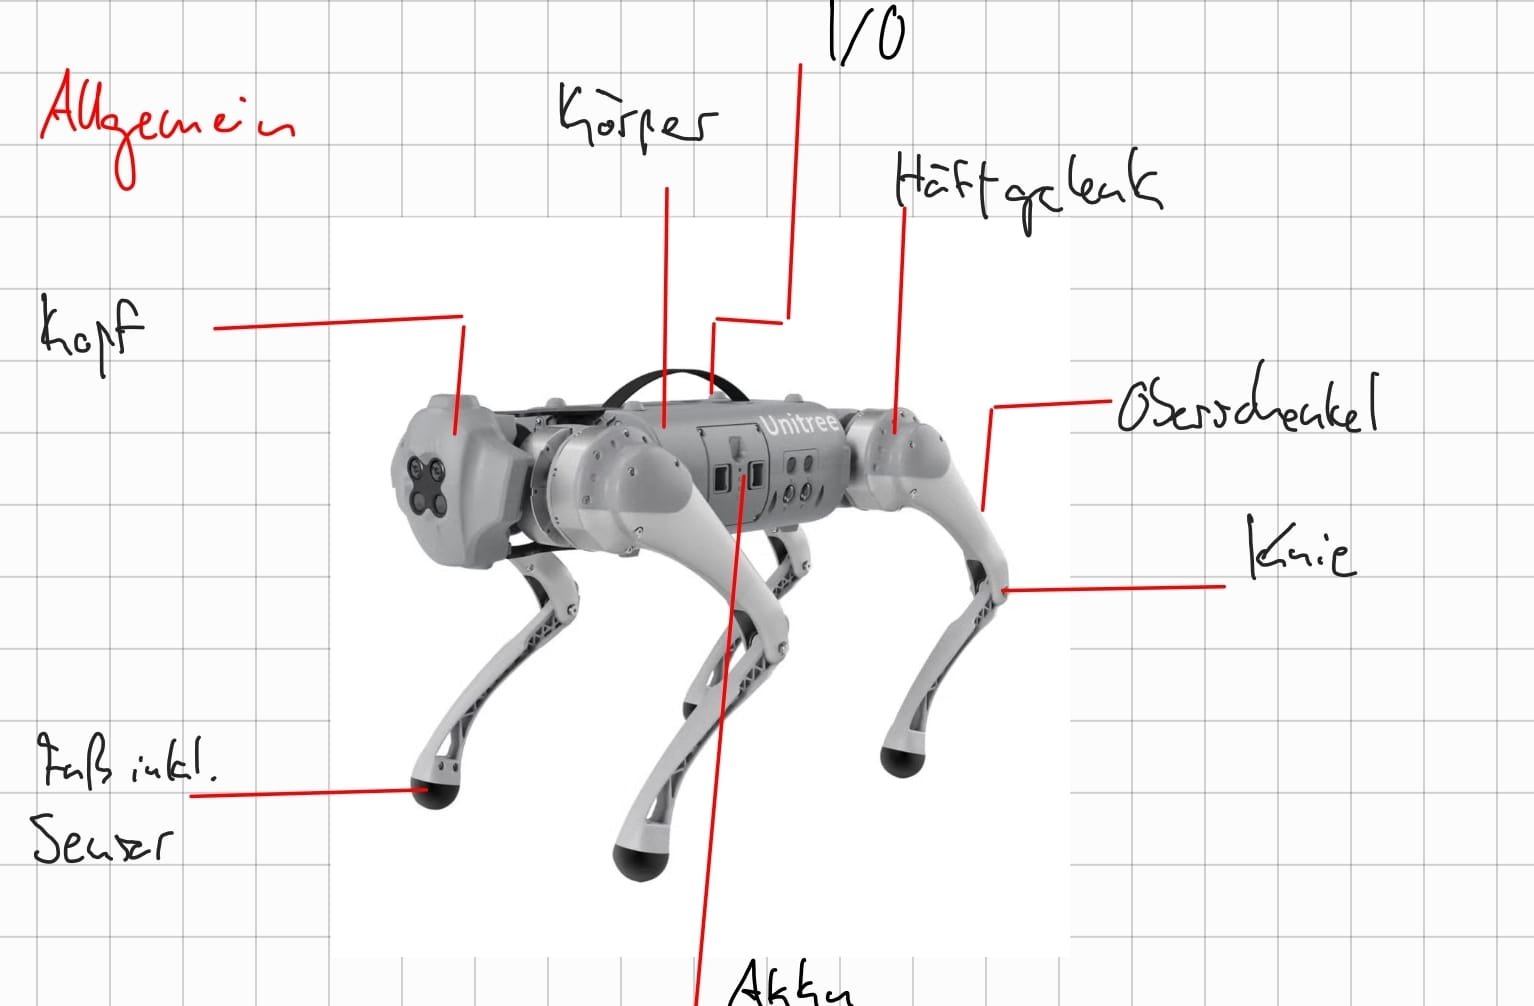
\includegraphics[width=\linewidth]{img/architektur/allgemein}}
    \caption{Überblick über den \gls{go1}}\label{fig:allgemeine_architektur}
\end{figure}

\subsubsection{Mechanische Komponenten}

\begin{figure}[h]
    \frame{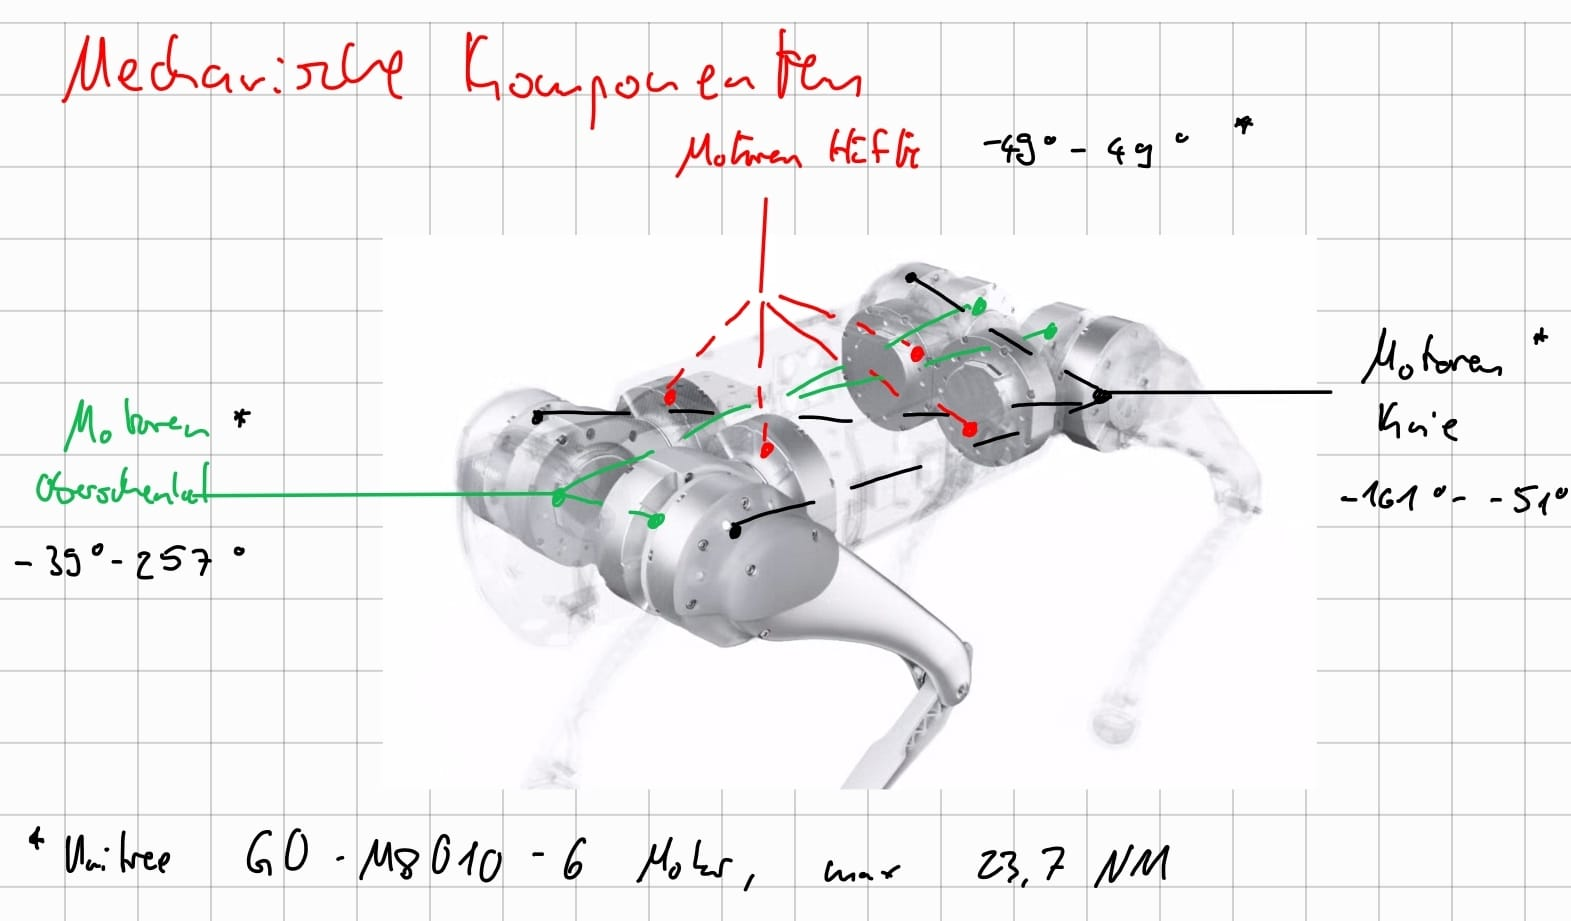
\includegraphics[width=\linewidth]{img/architektur/mechanische_komponenten}}
    \caption{Mechanische Komponenten des \gls{go1}}\label{fig:mechanische_komponenten}
\end{figure}

\subsubsection{Hardware und Sensorik}

\begin{figure}[h]
    \frame{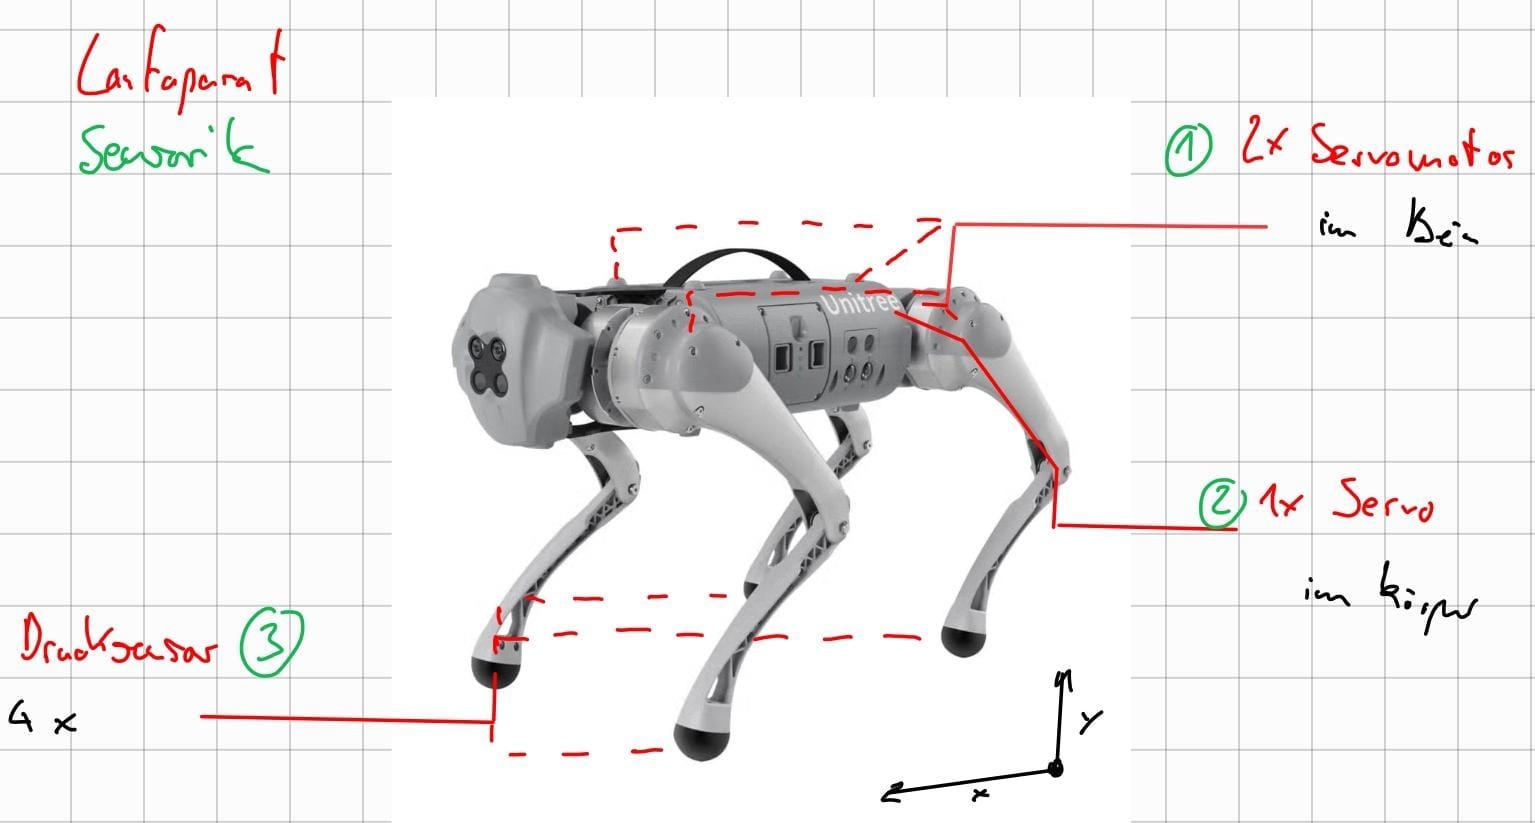
\includegraphics[width=\linewidth]{img/architektur/laufaparat}}
    \caption{Sensorik und Daten des Laufaparats}\label{fig:laufaparat}
\end{figure}

\begin{figure}[h]
    \frame{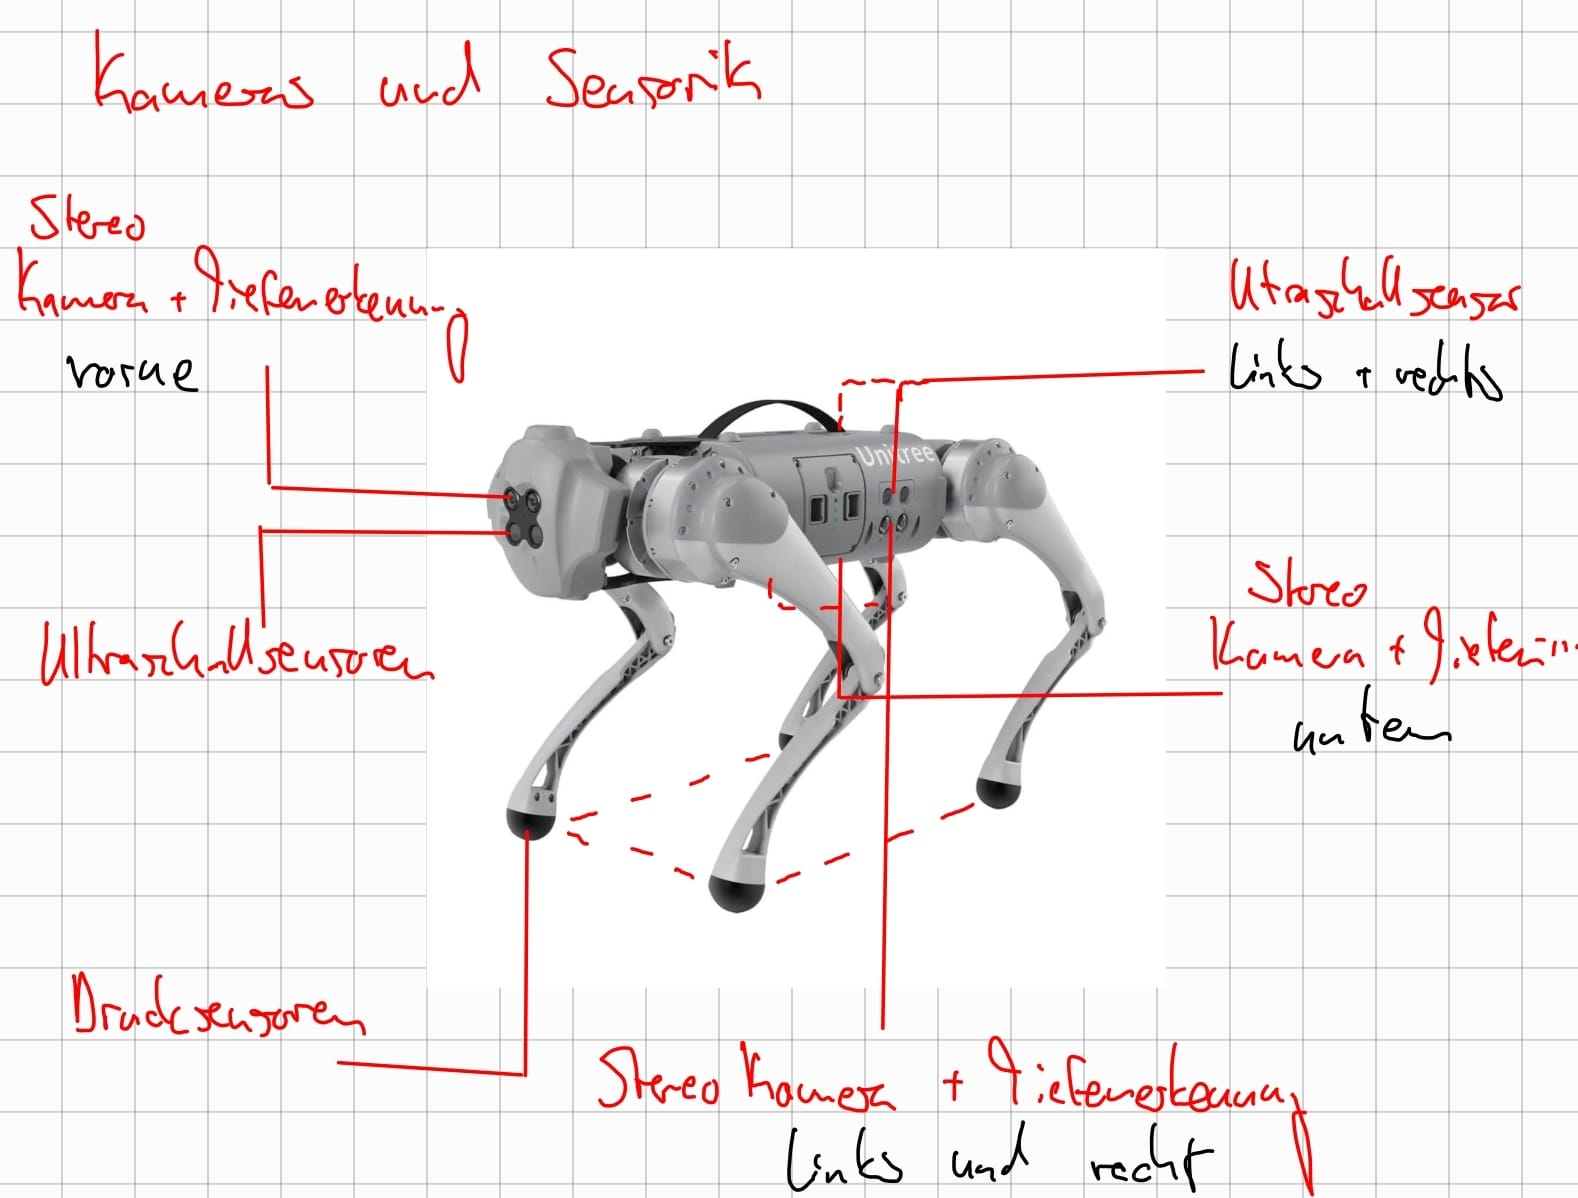
\includegraphics[width=\linewidth]{img/architektur/kameras_sensorik}}
    \caption{Darrstellung der verbauten Kamera und Sensorik}\label{fig:kameras_sensorik}
\end{figure}

\begin{figure}[h]
    \frame{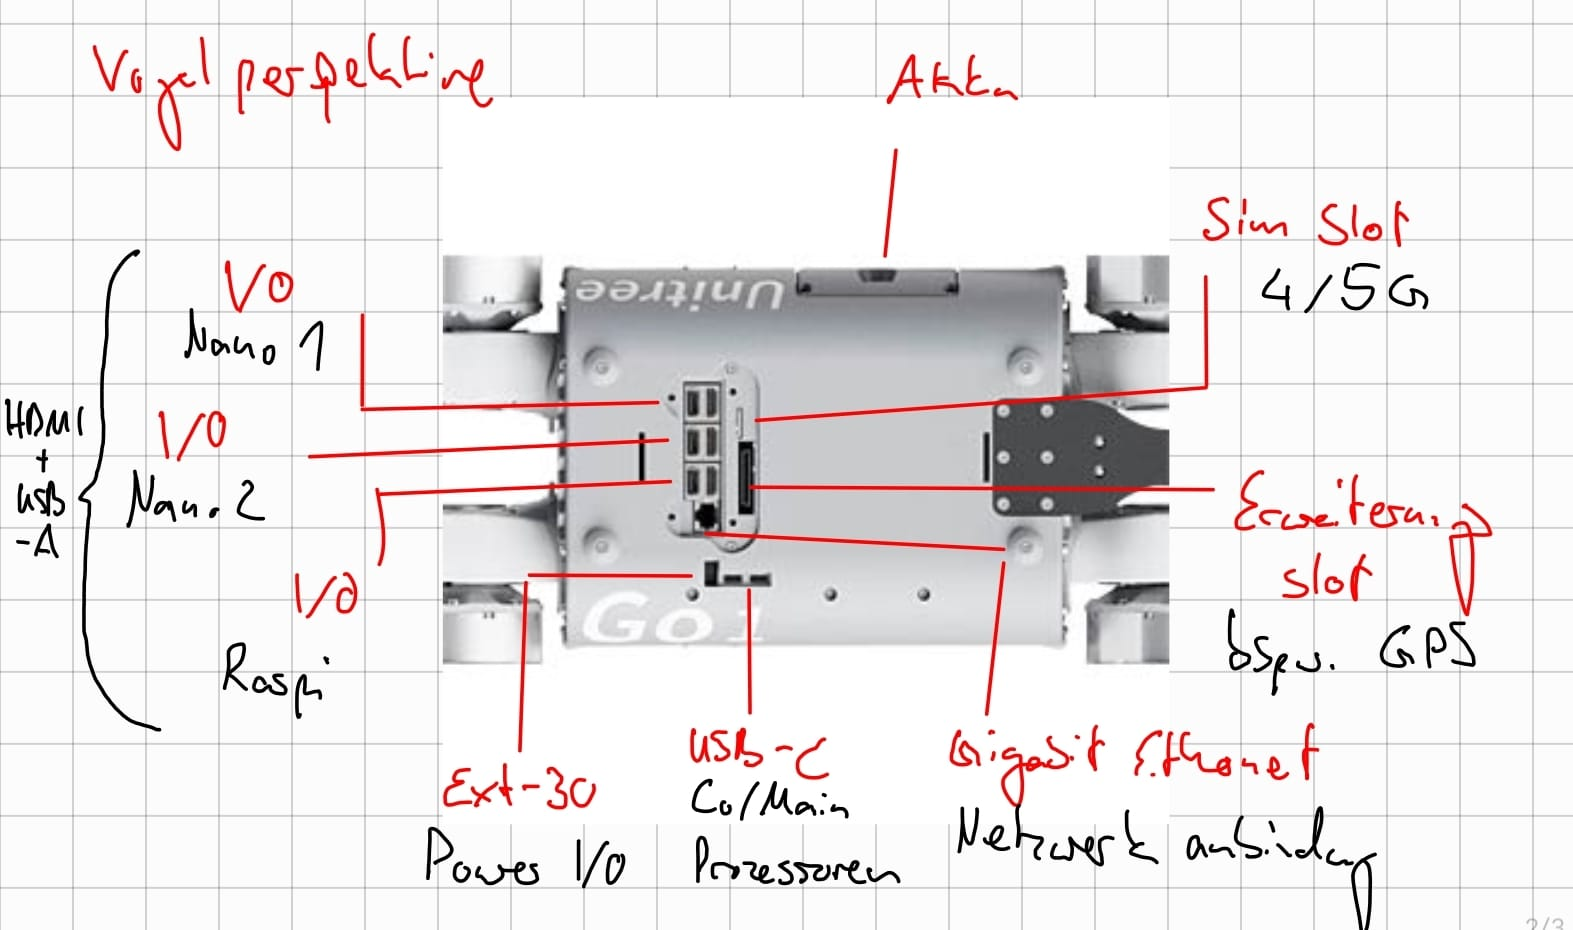
\includegraphics[width=\linewidth]{img/architektur/hardware}}
    \caption{Vogelperspektive mit Hardware}\label{fig:hardware}
\end{figure}

\subsection{Inbetriebnahme}

\subsection{Hardware Architektur}
\subsubsection{Überblick}
\subsubsection{Kernelemente}
\subsubsection{Spezialisierte Hardware}
\subsubsection{Netzwerk}

\subsection{Limitierungen}
\subsubsection{Rechenleistung}
\subsubsection{Physische Limitierungen}